In this chapter are collected my interpretations of the results obtained, in particular by Borda Count algorithm and Pearson index. Interpretation of the results could be shared between the 2 target variable or specific to one of them.

\section{Feature Selection Results}
In this section the results obtained for each target variable selected are explained in relation to the:
\begin{itemize}
    \item votes received through Borda Count algorithm;
    \item positive or negative correlation assumed in the filter methods;
    \item confirmation in literature where a given correlation occurred; 
\end{itemize}
Similarity between the tests run for each target variable are visible for many factors that influence both particulate matter and ammonia (figure \ref{fig:pearson_general}).
This can be observed by the similarity of the both positive and negative correlation from indexes from filter methods (such as Pearson, figure \ref{fig:pearson_general}). 
For instance, DTM average elevation and slope ('h\_mean' and 'slope\_mean' respectively) are correlated in the same way in test of both target variables, since air pollution affects more urban than mountain areas.
A general condition present in most of the tests run (which are available in the Appendix \ref{chap:appendix}) is the influence with respect to meteorological parameters.
For instance, pollutants are negatively correlated to wind speed ('e\_wind'), since their concentration tends to turn down with it. Wind is a marker for the horizontal transport of air pollutants. Pressure also contributes to them ('press'), since it causes stable atmospheric conditions that make pollutants harder to be disseminated. 
In addition, the findings didn't find consistent differences if Alpes and Prealpes zones are included or not. The only slight diversity found is about the pollutant, soil, and vegetation variables, which tends to be generally higher if mountains are excluded.

\begin{comment}
 is a moderate correlation with temperature. 
Air temperature ('temp\_2m' and 'temp\_int') increases with global radiation, while pollutants significantly decreased\cite{li2015particulate} in many test cases. The negative correlation between pollution and air humidity can also be observed (air\_hum\_int).
Under increased humidity conditions, PM and ammonia may be prone to a washout mechanism due to moisture in the air, causing a particulate reduction\cite{biglari2017relationship}.\\
For instance, AOD ('aod\_047' and 'aod\_055') has a strong correlation with pollutants (more with PM2.5 than ammonia) , due to the fact that they are suspension of a solid or liquid particles in the air. AOD in fact measure the atmospheric aerosols
\end{comment}
\begin{figure}[H]
\centering
\subfloat[pm25\_st as target variable.]{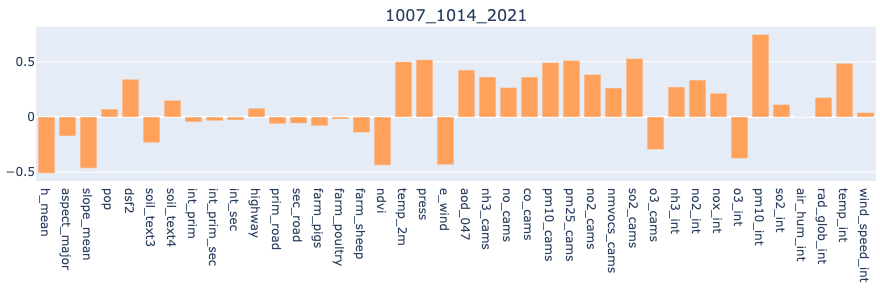
\includegraphics[scale =0.45]{images/tests/pm25pearson_october_0_01_mountains.png}}\\
\subfloat[nh3\_st as target variable.]{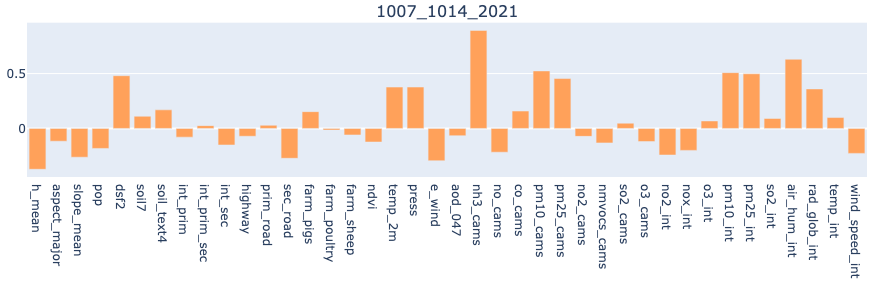
\includegraphics[scale =0.45]{images/tests/nh3_pearson_october_0_01_mountains.png}}
\caption{Pearson index results obtained in the period between 7-14 October with 1km resolution including mountains.}
\label{fig:pearson_general}
\end{figure}
\subsection{PM2.5 as target variable}
Fine particulate matter (PM2.5) is one of the most common air pollutants in our environment. 
It comes primarily from transport vehicle (such as car, truck and bus), industry, burning of fuels and household activities.\\ \par
During the 5 periods, it has been shown that PM2.5, as the other pollutants, changes over time. Air pollution change accordingly to the type of climate and atmospheric conditions.\\
\begin{comment}
In the tests is also visible the score obtained by ozone ('o3\_int') which tends to be positively correlated in the period between 18 and 25 April.\\
This, as mentioned before, is possibly due to their common precursors, such as nitrogen oxides and volatile organic compounds and their simultaneous generation in photochemical reactions. \\
\end{comment}
Air pollution analysis can confirm the presence of a high amount in the winter and heating season and a low quantity in the summer months\cite{cichowicz2017dispersion}. This is not applied to the ozone ('o3\_int' and 'o3\_cams'), which should be, on the contrary, higher during summer due to combination of heat and sunlight which reacts with nitrogen oxides (NOx) and volatile organic compounds. Indeed, ozone receive in the results many votes for its negative correlation (the highest in summer period), due to the fact that is inversely related to PM2.5.\\
By the bar plots attached in the figure \ref{fig:fs_pm25}, it is clear that most of the pollutants have a strong or moderate correlation with PM2.5. 
It can be shown in figure \ref{fig:pearson_general} that the entire set of pollutants variables is almost all positively correlated to it.
In particular, PM10 provided by ARPA and CAMS, in the various test executed is one of the most correlated pollutant. Indeed, 'pm10\_int' and 'pm10\_cams' have always an high number of vote. A strong positive correlation between PM2.5 and PM10 is also demonstrated in the literature\cite{zhou2016concentrations}.
Another variable which received a strong number of votes is the PM2.5 modelled by CAMS ('pm25\_cams'). 
Both variables, in fact, measure the same pollution phenomena as the target variables. This finding make us understand how both describe the same pollution phenomena, moving to the same direction. Indeed, the correlation coefficient between them is close to 1 in all tests executed.
It's visible a correlation with nitrogen dioxide('no2\_int'), a strong greenhouse gas which is related, as particulate matter, to biomass burning, industrial processes, households and road transport\cite{zellner2000john}\cite{maranzano2022air}.
From nitrogen dioxide derives also the chemical relation with the other nitrogen oxides ('nox\_int'), such as nitrogen monoxide ('no\_int') and carbon monoxide ('co\_int', 'co\_cams, 'co\_s5p'). This could be explained by the fact that they contribute as a secondary pollutant to PM2.5 formation \cite{xie2015spatiotemporal}.
\\
Observing the results regarding intense agriculture, it's evident that ammonia ('nh3\_int' and 'nh3\_cams') received as PM10 most votes of all in spring period due to its strong positively correlation. 
This happens because NH3 can react in the atmosphere to form ammonium salts in the presence of acid species\cite{viatte2021ammonia}.
We can assume that the main source of ammonia emission is intense agriculture, since it was responsible for 92\% of the total by EEA country members in 2017\cite{maranzano2022air}.\\
Indeed, during this periods, application of fertilizer contribute to ammonia and particulate matter.
Significantly more fertilizer is applied in the spring than in the summer and winter season due to crop cycles\cite{goebes2003ammonia}.
Therefore, we can assume that intense agriculture is one of the factors that influence the formation of PM2.5, with the greatest contribution during a certain period of the year.
\begin{figure}[H]
\centering
\subfloat[Borda Count algorithm results.]{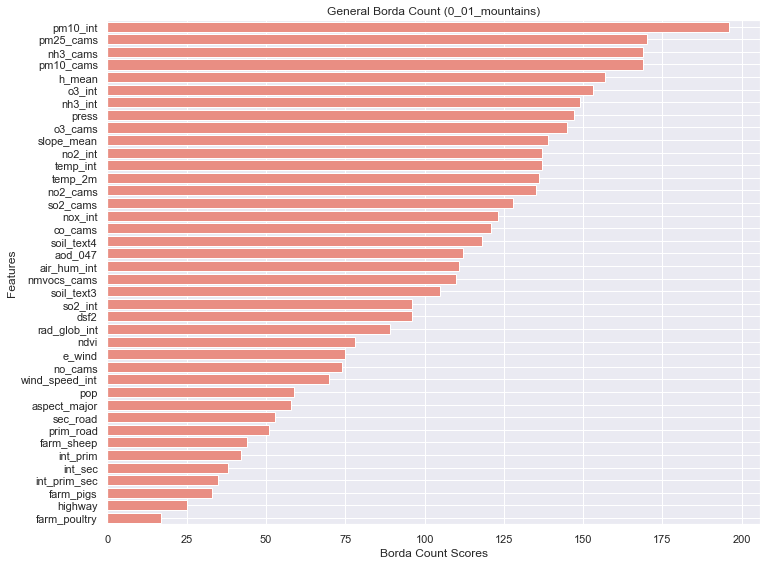
\includegraphics[scale =0.45]{images/tests/0_01_mountainspm25_st.png}}\\
\subfloat[Pearson index results in the  24-31 March and 18-25 April periods.]{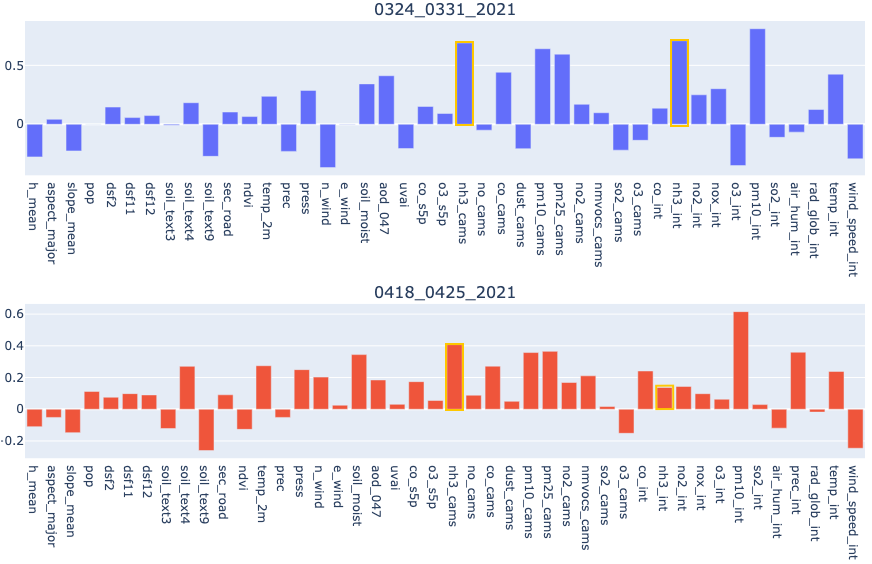
\includegraphics[scale =0.40]{images/tests/ammonia_effect_on_pm25_001mountains.png}}
\caption{FS results assuming PM2.5 as target variable with 10 Km resolution including mountains. In the figure (a) it is possible to observe the features ordered in decreasing order with respect to the votes received by Borda-Count algorithm. Figure (b) highlights the positive correlation assumed by ammonia variables in the spring period. }
\label{fig:fs_pm25}
\end{figure}
\subsection{NH3 as target variable}
Ammonia (NH3) is a reactive and soluble alkaline gas. It is one of the main sources of nitrogen pollution and comes from natural and anthropogenic sources, such as agriculture.
The process of ammonia evaporation commonly takes place when nitrogen is originated by urea of animal livestock, and fertilize. 
In the results obtained along the five periods, the ammonia provided by the CAMS model ('nh3\_cams') stands out, because it is strongly correlated, represents the same pollutant as well.
We can observe in figure \ref{fig:fs_nh3} also variable related to PM10 and PM2.5 ('pm10\_int', 'pm10\_cams','pm25\_int' and 'pm25\_cams'), because ammonia contribute for the formation of secondary particulate matter \cite{dai2019concentrations}\cite{zhu2015sources}.\\
Correlation of ammonia with respect to intensive agricultural should be feasible by the high positive correlation with agricultural areas (modelled by 'dsf2' variable), in particular used for maize cultivation ('siarl9') .\\
It's observable also the votes received by the variable that models the soil moisture, always with a positive correlation with respect to the target variable. This could be explained by the abundance of ammonia-oxidizing bacteria that increase with soil moisture \cite{avrahami2007response}.  
Other important weighted features are the ones related to intense farming ('farms' and 'farm\_pigs') which are responsible for ammonia release thanks to chemical reaction of urea.
In fact, animal urine and feces imply the release of ammonia and methane in the atmosphere, respectively\cite{saggar2004review}.
\begin{comment}
Indeed, methane ('ch4\_s5p') has a meaningful positive correlation with respect to NH3).\\.\\
It can be viewed also how road infrastructure variables contribute to ammonia. In particular the correlation between them is negative, since ammonia emission from agriculture occurs usually far from urban and traffic areas.\\
These effects are more visible in the configuration obtained by excluding the mountains zones, where pollutant effects are less visible.
\end{comment}
So we can suggest that ammonia in Lombardy should be very related to the use of fertilizer in agriculture areas and animal livestock in farms.
\bigbreak
\pagebreak
\clearpage
\begin{figure}[H]
\centering
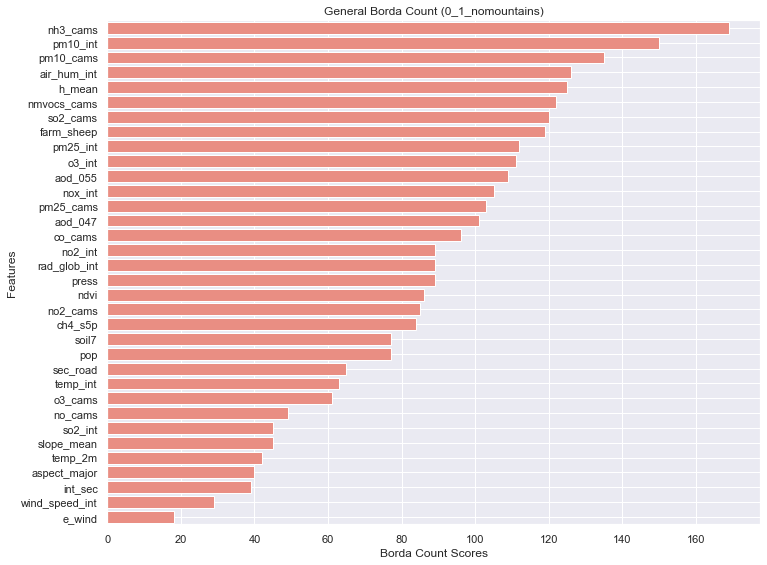
\includegraphics[scale =0.50]{images/tests/0_1_nomountainsnh3_st.png}
\caption{FS results obtained with Ammonia (NH3) as target variable with 1 Km resolution excluding mountains.}
\label{fig:fs_nh3}
\end{figure}
So overall, the results obtained in feature selection demonstrate two things.  
First, fine particulate should be very correlated with ammonia in the planting period (spring). Second, ammonia is strictly related to agriculture and farming activity, in accordance with previous studies.

\section{Data Modelling Results}
In this section are collected the interpretation of the ML models results, paying attention not only on the results achieved by the ARPA and CAMS models, but also on how feature selection could improve performance results. 
\subsection{Interpretation of validation results with ARPA sensor}
Models assure a consistent accuracy.
The errors obtained in the results by the validation through particle matter decrease as a function of the higher resolution.
Higher resolution, as a matter of fact, implies a larger number of sample for training and so a better accuracy as consequence.
Instead, in the models for ammonia estimation there are no relevant differences between the 2 resolutions.
With PM2.5 as target variable at 10 km resolution there is a lower statistical accuracy than at 1km, with MAE respectively around 1 and 0.5 ug/m\textsuperscript{3}(Table \ref{tab:res1km}). 
\begin{table}[H]
\begin{tabular}{lrrrrr}
\toprule
  &  24/03-31/03 &  18/04-25/04 &  17/07-24/07 &  3/09-10/09 &  7/10-14/10 \\
\midrule
  MAE\_sensor &        1.448 &        1.093 &        0.646 &       0.898 &       0.841 \\
RMSE\_sensor &        1.940 &        1.362 &        0.868 &       1.165 &       1.080 \\
 MSE\_sensor &        3.772 &        1.874 &        0.776 &       1.376 &       1.197 \\
  R2\_sensor &        0.872 &        0.766 &        0.683 &       0.870 &       0.793 \\
\bottomrule
\end{tabular}
\caption{Random Forest prediction for PM2.5 at 10 km, excluding zones with mountains.}
\end{table}
\begin{table}[H]
\begin{tabular}{lrrrrr}
\toprule
  &  24/03-31/03 &  18/04-25/04 &  17/07-24/07 &  3/09-10/09 &  7/10-14/10 \\
\midrule
  MAE\_sensor &        0.251 &        0.186 &        0.147 &       0.172 &       0.132 \\
RMSE\_sensor &        0.503 &        0.361 &        0.255 &       0.285 &       0.240 \\
 MSE\_sensor &        0.283 &        0.138 &        0.066 &       0.084 &       0.059 \\
  R2\_sensor &        0.992 &        0.985 &        0.981 &       0.994 &       0.993 \\
\bottomrule
\end{tabular}
\caption{Random Forest prediction for PM2.5 at 1 km, including zones with mountains.}
\label{tab:res1km}
\end{table}

\begin{table}[H]
\begin{tabular}{lrrrrr}
\toprule
  &  24/03-31/03 &  18/04-25/04 &  17/07-24/07 &  3/09-10/09 &  7/10-14/10 \\
\midrule
 MAE\_sensor &        0.483 &        0.280 &        0.526 &       0.939 &       0.386 \\
RMSE\_sensor &        0.993 &        0.558 &        1.184 &       2.316 &       0.860 \\
 MSE\_sensor &        1.199 &        0.430 &        1.556 &       6.147 &       1.121 \\
  R2\_sensor &        0.997 &        0.992 &        0.994 &       0.987 &       0.990 \\
\bottomrule
\end{tabular}
\caption{Random Forest prediction for NH3 at 1 km, excluding zones with mountains.}
\label{tab:nh3RF}
\end{table}
\begin{table}[H]
\begin{tabular}{lrrrrr}
\toprule
  &  24/03-31/03 &  18/04-25/04 &  17/07-24/07 &  3/09-10/09 &  7/10-14/10 \\
\midrule
 MAE\_sensor &        1.904 &        2.287 &        3.126 &       2.743 &       3.146 \\
RMSE\_sensor &        2.570 &        3.341 &        4.205 &       3.841 &       4.465 \\
 MSE\_sensor &        6.867 &       11.579 &       18.068 &      16.405 &      21.579 \\
  R2\_sensor &        0.984 &        0.800 &        0.927 &       0.965 &       0.852 \\
\bottomrule
\end{tabular}
\caption{Neural Network prediction for NH3 at 1 km, excluding zones with mountains.}
\label{tab:nh3NN}
\end{table}
In the model for the estimation of ammonia, instead, this error is clearly higher(Table \ref{tab:nh3RF}).
Nevertheless, results are substantially accurate as well. 
This difference should be given by a different number of ground sensors for each pollutant. In fact, the sample for the measurement of particulate matter is larger than the one for ammonia (Figure \ref{fig:comparison-sensors}).
\begin{figure}[H] 
    \centering
    \subfloat[PM2.5 as target variable.]{%
        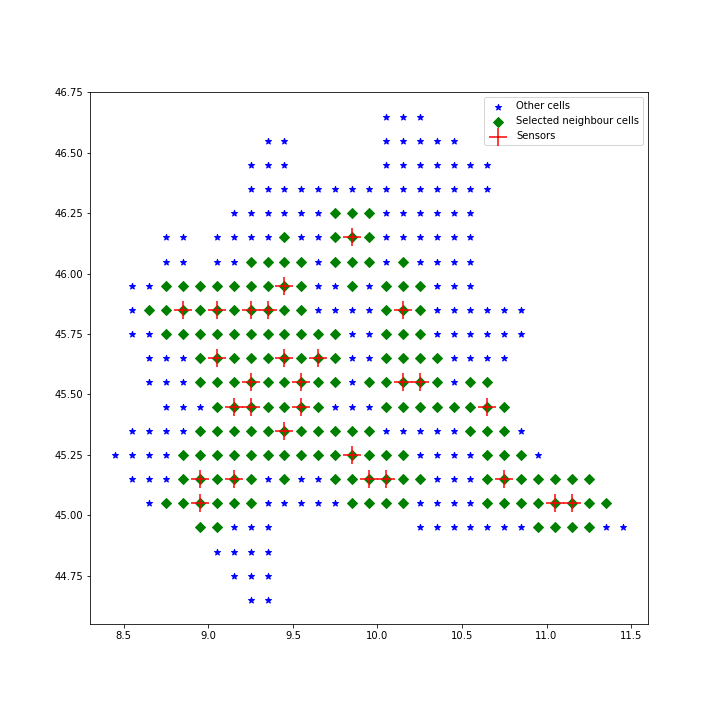
\includegraphics[width=0.5\textwidth]{images/pm25_sensors.png}%
        %
        }%
    \hfill%
    \subfloat[NH3 as target variable.]{%
        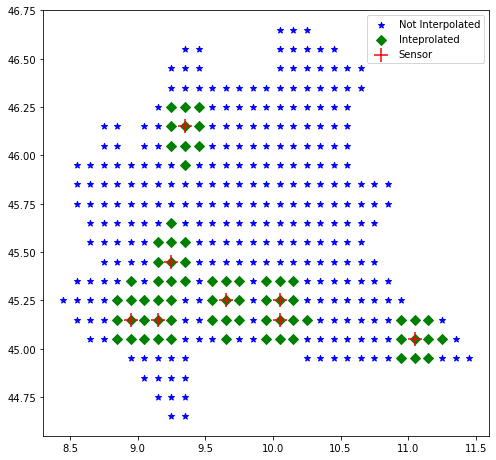
\includegraphics[width=0.5\textwidth]{images/nh3_sensors.png}%
        %
        }%
    \caption{In these images are shown the observations at 10km resolution of each different target variable used in this case of study. The legend shows whether the cell has an interpolated value with KNN or not. In addition ground sensor from which interpolation is performed are added. 
    The sample number passed from 28 to 173 for PM2.5 as target variable and from 8 to 69 for NH3.}
    \label{fig:comparison-sensors}
\end{figure}

We can observe that generally the Random Forest model makes more accurate predictions than the Neural Network by Keras (Tables \ref{tab:nh3RF} and \ref{tab:nh3NN}). 
This may be due to the fact that the RF algorithm uses the ensemble learning method for regression, a technique that joins estimation from multiple models to have more accurate predictions than a single model. 
R\textsuperscript{2} in each test assumes a positive value, meaning that the pollutants take in consideration in this case of study can be explained by the regression models. 
\subsection{Comparison with CAMS model}
The comparison between the models of my results and CAMS data shows how values are very far from them. MAE for PM2.5 values is around 5 while for ammonia around 10 ug/m\textsuperscript{3}. 
Another difference between the two models is the R\textsuperscript{2} value which assumes a negative value in most cases. It proves the presence of a big difference between training and test values. 


\begin{table}[H]
\begin{tabular}{lrrrrr}
\toprule
  &  24/03-31/03 &  18/04-25/04 &  17/07-24/07 &  3/09-10/09 &  7/10-14/10 \\
\midrule
  MAE\_cams &        7.800 &        6.556 &        2.110 &       3.060 &       3.478 \\
  RMSE\_cams &        9.262 &        7.571 &        2.745 &       3.623 &       4.059 \\
   MSE\_cams &       86.279 &       57.593 &        7.548 &      13.266 &      16.591 \\
    R2\_cams &       -2.147 &       -7.492 &       -2.846 &      -0.258 &      -1.096 \\
\bottomrule
\end{tabular}
\caption{Random Forest prediction for PM2.5 at 1 km, including zones with mountains.}
\end{table}
\begin{table}[H]
\begin{tabular}{lrrrrr}
\toprule
  &  24/03-31/03 &  18/04-25/04 &  17/07-24/07 &  3/09-10/09 &  7/10-14/10 \\
\midrule
   MAE\_cams &       18.401 &       10.414 &       11.746 &      14.180 &      12.012 \\
  RMSE\_cams &       19.196 &       12.126 &       17.744 &      21.241 &      13.697 \\
   MSE\_cams &      368.858 &      147.652 &      323.418 &     456.145 &     188.650 \\
    R2\_cams &        0.136 &       -1.511 &       -0.158 &      -0.001 &      -0.060 \\
\bottomrule
\end{tabular}
\caption{Random Forest prediction for NH3 at 1 km, excluding zones with mountains.}
\end{table}
These results are in contrast with the FS results, where the correlation between the ARPA values (target variable) and the CAMS models is one of the strongest.
From this results we hypothesize that both pm25\_st / nh3\_st and pm25\_cams / nh3\_cams variables shape the same pollution phenomenon having the same behavior, but between them there would be a bias.\\
Obviously the model of Copernicus Atmosphere Monitoring Service provide different results by one obtained by me, since is build very differently. CAMS is built through ensemble median, averaged by eleven European air quality forecasting systems. Therefore, the median model should perform better than the individual model products\cite{riccio2007seeking}; 
Anyway, through information collected on the Copernicus website, only a limited number of ground observations are detected in the Italian territory. As can be seen in figure \ref{fig:cams} in Italy there is only 1 observation in Sardinia for PM2.5 detection. Nothing was found for Ammonia.
\begin{figure}[H]
    \centering
    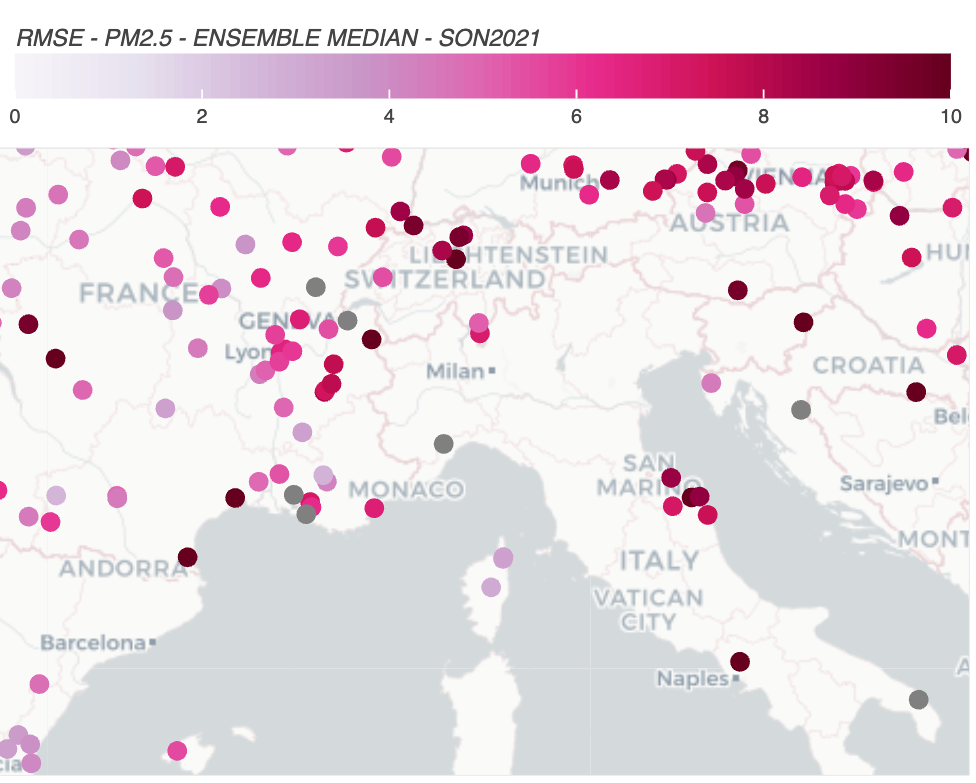
\includegraphics[scale=0.2]{images/cams_obs.png}
    \caption{The following map include a set of points layers representing the forecast performance of the station used by the ensemble median model of CAMS. In particular the RMSE of them is shown\cite{camsobs}. 
}
    \label{fig:cams}
\end{figure}

So, by the validation results and the larger number of ground observations provided by ARPA in this data collection, this model should perform better in this local scale.
\bigbreak
Based on these results, we can point out that Random Forest is more precise than the  Neural Network model and that the performance is higher for particulate matter than ammonia estimation.
Random Forest indeed is one the most preferred also in literature prediction model for its easy configuration.
\subsection{Importance of the FS}
The underlying tables provide model results respectively in 2 case:
\begin{itemize}
    \item the selection of variable is performed by Feature Selection procedure;
    \item the selection of variable is performed by a random function (for doing this was used the Pandas.sample method);
\end{itemize}
It can be observed that feature selection is meaningful for the pre-processing phase, since aims at discarding eventually useless variables and to take only the ones really relevant to the target variable. In the results obtained we can detected that selection of variable with FS assume a key role for sample of small size. 
Indeed, in the tests with resolution 10 Km model there is a feasible difference between the data trained by variable from FS and the ones chosen randomly (Table \ref{fig:importance10km}). 
This gap becomes negligible with higher resolution (Table \ref{fig:importance1km}).
This is implied by the fact that more the training size is sufficient, less a feature selection procedure improve the accuracy\cite{chu2012does}.
\newline
In conclusion, the difference between the results of this test and the ones run for each period shows also the presence of overfitting in my models. Indeed, results obtained with temporal hold-out validation (in particular for  R\textsuperscript{2}) shows how the \acrshort{rf} model can't make accurate predictions about new data (which comes from a different period).  

\begin{table}[H]
\centering
\subfloat[10 km resolution.]
{\begin{tabular}{lrr}
\toprule
 &  With FS & Without FS \\
  \midrule
 MAE\_sensor &        2.076  &        2.735 \\
RMSE\_sensor &        2.579 &        3.285  \\
 MSE\_sensor &        6.650  &        10.794 \\
  R2\_sensor &        0.168  &         -0.349\\
\end{tabular}
\label{fig:importance10km}}
\\
\subfloat[1 km resolution.]
{\begin{tabular}{lrr}
\toprule
& With FS &  Without FS\\
\midrule
 MAE\_sensor &        2.634 &        2.992 \\
RMSE\_sensor &        3.170  &        3.832\\
 MSE\_sensor &        10.046 &        14.687  \\
  R2\_sensor &        -0.220 &        -0.784 \\
 \label{fig:importance1km}
\end{tabular}}
\caption{Random Forest prediction for PM2.5, including zones with mountains using or not FS.}
\end{table}



\begin{comment}
ps://www.sciencedirect.com/topics/agricultural-and-biological-sciences/agricultural-pollution 
https://pure.iiasa.ac.at/id/eprint/14769/1/Reduction%20of%20NH3%20emissions%20from%20agriculture%20in%20the%20Hai%20River%20Basin%20in%20China.pdf

https://towardsdatascience.com/batch-mini-batch-stochastic-gradient-descent-7a62ecba642a
\end{comment}
